\chapter{Synthèse asymétrique}\label{ch:b3:asymmetric-synthesis}

La L-DOPA, le médicament qui atténue les symptômes de la maladie de
Parkinson, fut dans les années 1970 le premier composé fabriqué
industriellement par \omterm{def:b3:asymmetric-synthesis:asymmetric-catalysis}{catalyse asymétrique}~: quelques grammes d'un complexe
chiral du rhodium, dissous avec un précurseur plan et achiral sous
dihydrogène, donnaient un produit dans lequel un énantiomère l'emportait
largement sur l'autre. Les deux énantiomères d'un médicament peuvent avoir
des effets complètement différents, parce que les récepteurs et les
\omterm{def:b3:complex-kinetics:enzyme}{enzymes} qu'ils rencontrent sont eux-mêmes chiraux. Ce chapitre mesure la
pureté énantiomérique, explique comment un environnement chiral choisit
entre deux chemins images l'un de l'autre dans un miroir, et passe en revue
les stratégies (\omterm{def:b3:asymmetric-synthesis:chiral-pool}{réservoir chiral}, auxiliaires, dédoublements, catalyseurs
métalliques et organiques) qui produisent des énantiomères purs.

\begin{recall}
Le volume de première année a défini la chiralité, les énantiomères, les
diastéréoisomères, les mélanges racémiques, le pouvoir rotatoire
spécifique, les règles CIP et les réactions stéréosélectives et
stéréospécifiques~; le volume de deuxième année, l'hydrogénation
catalytique, l'époxydation, la dihydroxylation, les imines, les énamines,
les énolates, l'aldolisation, l'annélation de Robinson et la
chromatographie. Le \cref{ch:b3:rate-theories} a donné l'\omterm{thm:b3:rate-theories:eyring}{équation
d'Eyring}, le \cref{ch:b3:homogeneous-catalysis} le cycle de Wilkinson, et
le \cref{ch:b3:point-groups} l'axe $C_2$.
\end{recall}

\begin{omfigure}
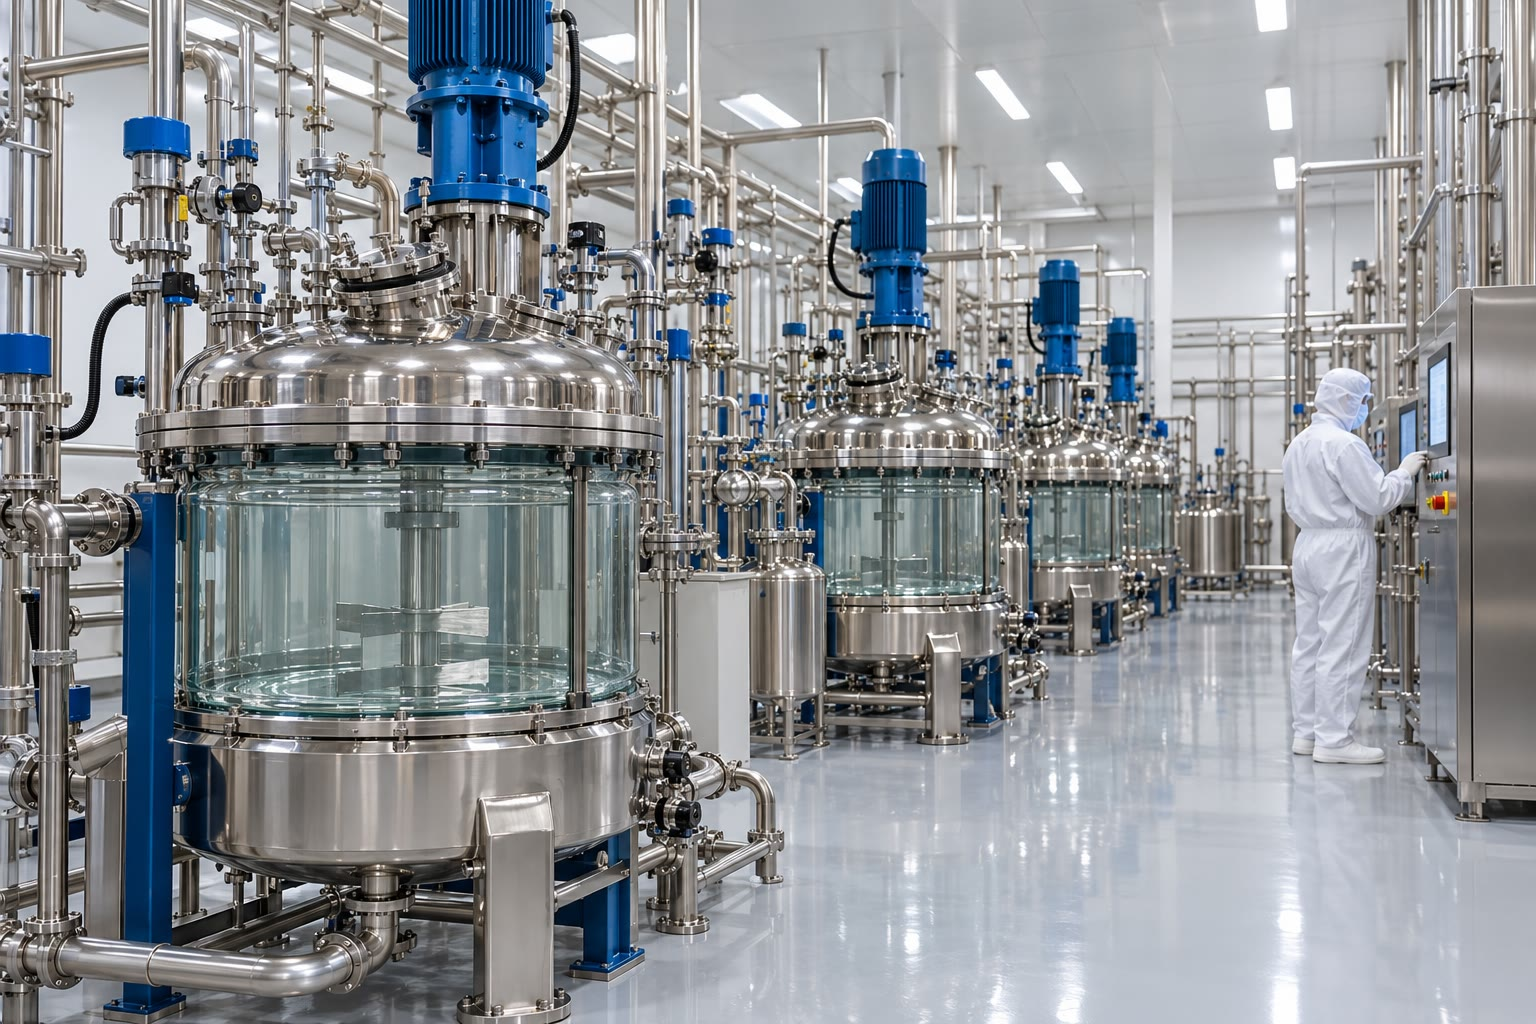
\includegraphics[width=0.58\linewidth]{images/book4/ai/b3-28-api-plant.jpg}

{\small Une halle de réacteurs émaillés dans une usine de principes actifs
pharmaceutiques. Beaucoup de ses produits sont des énantiomères purs,
obtenus par catalyse ou par dédoublement et contrôlés par chromatographie
chirale.}
\end{omfigure}

\section{Mesurer la pureté énantiomérique}

\begin{definition}[Excès énantiomérique]\label{def:b3:asymmetric-synthesis:ee}
Pour un mélange d'énantiomères en quantités $n_R \ge n_S$, l'\emph{excès énantiomérique}\index{exces enantiomerique@excès énantiomérique} vaut $\mathrm{ee} = (n_R - n_S)/(n_R + n_S)$ et le \emph{rapport énantiomérique}
\index{rapport enantiomerique@rapport énantiomérique} $\mathrm{er} = n_R/n_S$~; pour des diastéréoisomères,
l'\emph{excès diastéréoisomérique}\index{exces diastereoisomerique@excès diastéréoisomérique} de se définit de la même
façon. La \emph{pureté optique}\index{purete optique@pureté optique} est le rapport du pouvoir
rotatoire spécifique d'un échantillon à celui de l'énantiomère pur.
\end{definition}

\begin{proposition}[ee et er]\label{prop:b3:asymmetric-synthesis:ee-er}
$\mathrm{ee} = (\mathrm{er} - 1)/(\mathrm{er} + 1)$ et $\mathrm{er} = (1 + \mathrm{ee})/(1 - \mathrm{ee})$.
\end{proposition}

\begin{proof}
On divise le numérateur et le dénominateur de $(n_R - n_S)/(n_R + n_S)$ par $n_S$~; la résolution
en er donne la seconde forme.
\end{proof}

Un ee de 90\,\% correspond à un er de 95\,:\,5, un ee de 98\,\% à un er de
99\,:\,1. La \omterm{def:b3:asymmetric-synthesis:ee}{pureté optique} n'est égale à l'ee que si le pouvoir rotatoire
est proportionnel à la composition~; les impuretés, le solvant, les effets
de concentration et les faibles pouvoirs rotatoires de nombreux composés la
rendent peu fiable, et l'ee se mesure en séparant les énantiomères.

\begin{method}[ee à partir d'un chromatogramme chiral]\label{met:b3:asymmetric-synthesis:ee-chromatogram}
\begin{enumerate}
  \item Injecter d'abord le racémique, pour identifier les deux pics et
        vérifier leur séparation (résolution à la ligne de base) et
        l'égalité de leurs aires.
  \item Injecter l'échantillon et intégrer les deux pics.
  \item Les énantiomères ont la même réponse dans un détecteur achiral,
        donc
        $\mathrm{ee} = (A_1 - A_2)/(A_1 + A_2)$~; attribuer les pics à l'aide d'un étalon énantiopur.
\end{enumerate}
\end{method}

\begin{omfigure}
\begin{tikzpicture}
\begin{axis}[name=a, width=0.48\linewidth, height=5.4cm, xmin=0, xmax=20, ymin=0, ymax=1.0,
  axis lines=left, xlabel={$\Delta\Delta G^\ddagger$ / \unit{kJ.mol^{-1}}}, ylabel={ee},
  tick label style={font=\scriptsize}, label style={font=\small}]
\addplot[omDef, thick] table[x=ddg, y=eeA] {figdata/out/bachelor-3-er-ddg.dat};
\addplot[omMeth, thick] table[x=ddg, y=eeB] {figdata/out/bachelor-3-er-ddg.dat};
\addplot[omThm, thick] table[x=ddg, y=eeC] {figdata/out/bachelor-3-er-ddg.dat};
\node[font=\scriptsize, omDef, anchor=west] at (axis cs:10,0.55) {\qty{-78}{\celsius}};
\node[font=\scriptsize, omMeth, anchor=west] at (axis cs:10,0.43) {\qty{0}{\celsius}};
\node[font=\scriptsize, omThm, anchor=west] at (axis cs:10,0.31) {\qty{25}{\celsius} (en bas)};
\end{axis}
\begin{axis}[at={(a.east)}, anchor=west, xshift=1.4cm, width=0.48\linewidth, height=5.4cm,
  xmin=7.5, xmax=9.5, ymin=0, axis lines=left, ytick=\empty,
  xlabel={temps de rétention / min}, ylabel={signal du détecteur},
  tick label style={font=\scriptsize}, label style={font=\small}]
\addplot[black, thick] table[x=t, y=y] {figdata/out/bachelor-3-er-ddg-b.dat};
\node[font=\scriptsize, anchor=south west] at (axis cs:8.3,250) {(\textit{R})~: 97.5};
\node[font=\scriptsize, anchor=south] at (axis cs:9.1,20) {(\textit{S})~: 2.5};
\end{axis}
\end{tikzpicture}

{\small À gauche~: \omterm{def:b3:asymmetric-synthesis:ee}{excès énantiomérique} en fonction de la différence des
\omterm{def:b3:rate-theories:activation}{enthalpies libres d'activation} des deux chemins concurrents, à trois
températures~: le même
$\Delta\Delta G^\ddagger$ donne un ee plus élevé à basse température. À droite~: un chromatogramme HPLC chiral,
aires des pics 97.5 et 2.5 (modèle)~: ee 95\,\%.}
\end{omfigure}

La RMN ne distingue les énantiomères que dans un environnement chiral~: un
agent de solvatation chiral forme des complexes diastéréoisomères éphémères
dont les signaux diffèrent, et un alcool ou une amine chiraux convertis en
leurs deux esters diastéréoisomères par l'acide de Mosher révèlent la
configuration par le motif des différences de déplacement.

\begin{method}[Configuration par les esters de Mosher, dans les grandes lignes]\label{met:b3:asymmetric-synthesis:mosher}
\begin{enumerate}
  \item Préparer les deux esters MTPA, (\textit{R}) et (\textit{S}), de l'alcool.
  \item Enregistrer leurs spectres de proton et calculer $\Delta\delta = \delta_S - \delta_R$ pour les protons de chaque
        côté du carbone carbinol.
  \item Dans la conformation préférée, le cycle phényle de l'acide blinde
        un côté~:
        les protons pour lesquels $\Delta\delta > 0$ sont d'un côté, ceux pour lesquels $\Delta\delta < 0$ de l'autre, ce qui
        place les deux substituants et donne la configuration.
\end{enumerate}
\end{method}

\section{Topicité et additions stéréosélectives}

\begin{definition}[Réactions stéréosélectives]\label{def:b3:asymmetric-synthesis:selective}
Une \emph{réaction énantiosélective}\index{reaction enantioselective@réaction énantiosélective} forme un
énantiomère d'un produit en excès par rapport à l'autre~; une \emph{réaction diastéréosélective}\index{reaction diastereoselective@réaction diastéréosélective} forme un diastéréoisomère en excès.
\end{definition}

\begin{definition}[Topicité]\label{def:b3:asymmetric-synthesis:topicity}
Deux groupes d'une molécule sont \emph{homotopes}\index{homotopes} lorsqu'une
rotation de la molécule les échange (remplacer l'un ou l'autre donne le
même composé), \emph{énantiotopes}\index{enantiotopes@énantiotopes} lorsque seule une
réflexion les échange (remplacer l'un ou l'autre donne des énantiomères),
et \emph{diastéréotopes}\index{diastereotopes@diastéréotopes} lorsqu'aucune \omterm{def:b3:point-groups:operation}{opération de
symétrie} ne les échange (remplacer l'un ou l'autre donne des
diastéréoisomères).
\end{definition}

Les deux hydrogènes d'un groupe $\ce{CH2}$ voisin d'un stéréocentre sont \omterm{def:b3:asymmetric-synthesis:topicity}{diastéréotopes}~: ils
ont des déplacements chimiques différents et se couplent entre eux, ce qui
explique qu'un tel groupe apparaisse souvent sous forme de deux signaux en
RMN.

\begin{definition}[Faces prochirales]\label{def:b3:asymmetric-synthesis:faces}
Un carbone trigonal portant trois substituants différents est \emph{prochiral}\index{prochiral}~:
l'addition d'un quatrième groupe, différent, crée un stéréocentre. Sa face
vue avec les trois substituants, par ordre de priorité CIP décroissante,
dans le sens horaire est la \emph{face Re}\index{face Re}~; dans le sens antihoraire, la \emph{face Si}\index{face Si}.
\end{definition}

\begin{omfigure}
\begin{tikzpicture}[font=\small, >=Stealth]
  \coordinate (c) at (0,0);
  \draw[thick, double, double distance=1.6pt] (c) -- (90:1.1) node[above] {O (1)};
  \draw[thick] (c) -- (210:1.1) node[below left] {$\ce{C6H5}$ (2)};
  \draw[thick] (c) -- (330:1.1) node[below right] {$\ce{CH3}$ (3)};
  \fill (c) circle (1.6pt);
  \draw[->, thick, omThm] (70:0.6) arc[start angle=70, end angle=200, radius=0.6];
  \node[font=\scriptsize, omThm, align=center] at (-1.9,0.75) {1 $\to$ 2 $\to$ 3\\ sens antihoraire~:\\ face \textit{Si}};
  \node[font=\scriptsize, align=left, anchor=west] at (2.6,0.4) {face tournée vers le lecteur~: \textit{Si}\\ face derrière la page~: \textit{Re}};
  \node[font=\scriptsize, align=left, anchor=west] at (2.6,-0.5) {hydrure ajouté par la face \textit{Re}\\ donne le (\textit{S})-1-phényléthanol};
\end{tikzpicture}

{\small Les faces de l'acétophénone. Vus de devant, les substituants du
carbone du carbonyle dans l'ordre CIP (O, phényle, méthyle) tournent dans
le sens antihoraire~: la face avant est \textit{Si}, la face arrière \textit{Re}.}
\end{omfigure}

\begin{method}[Attribuer les faces Re et Si]\label{met:b3:asymmetric-synthesis:re-si}
\begin{enumerate}
  \item Classer les trois substituants de l'atome trigonal selon les règles
        CIP (une double liaison compte son partenaire deux fois).
  \item Regarder la face considérée, le plan trigonal étant dans le plan
        de la page.
  \item Sens horaire 1 $\to$ 2 $\to$ 3~: \textit{Re}~; sens antihoraire~: \textit{Si}.
  \item Pour nommer le produit, ajouter le nouveau groupe vers
        l'observateur et appliquer les règles CIP au nouveau stéréocentre~;
        une attaque Re ne donne pas toujours \textit{R}.
\end{enumerate}
\end{method}

\begin{definition}[Modèle de Felkin--Anh et contrôle par chélation]\label{def:b3:asymmetric-synthesis:felkin}
Le \emph{modèle de Felkin--Anh}\index{modele de Felkin--Anh@modèle de Felkin--Anh} prévoit le
diastéréoisomère majoritaire d'une addition nucléophile sur un groupe
carbonyle voisin d'un stéréocentre~: le plus gros groupe de ce centre se
place perpendiculairement au plan du carbonyle, et le nucléophile approche
en anti par rapport à lui, en passant près du plus petit groupe, selon la
trajectoire de Bürgi--Dunitz. Sous \emph{contrôle par chélation}\index{controle par chelation@contrôle par chélation}, un
ion métallique lié à la fois à l'oxygène du carbonyle et à un groupe
donneur du stéréocentre bloque la conformation, et le nucléophile
s'additionne sur la face la moins encombrée du cycle chélate.
\end{definition}

\begin{proposition}[Sélectivité de Felkin--Anh]\label{prop:b3:asymmetric-synthesis:felkin}
Pour un aldéhyde ou une cétone $\alpha$-chiral sans groupe chélatant, le produit majoritaire
est celui que prévoit le \omterm{def:b3:asymmetric-synthesis:felkin}{modèle de Felkin--Anh} (un modèle empirique,
étayé par le calcul). \admitted
\end{proposition}

\begin{omfigure}
\begin{tikzpicture}[font=\small, >=Stealth]
  \foreach \a/\lab in {90/L, 330/M, 210/S} {
    \draw[line width=0.8pt] (\a:0.55) -- (\a:1.1) node[pos=1.3] {\lab};
  }
  \fill[white] (0,0) circle (0.55);
  \draw[line width=0.8pt] (0,0) circle (0.55);
  \draw[line width=0.8pt, double, double distance=1.4pt] (0,0) -- (0:1.1) node[right] {O};
  \draw[line width=0.8pt] (0,0) -- (180:1.1) node[left] {R};
  \draw[->, very thick, omThm] (250:2.2) -- (250:0.25);
  \node[omThm, anchor=north] at (250:2.25) {Nu$^-$};
  \node[font=\scriptsize, align=left, anchor=west] at (1.7,-1.0) {Nu$^-$ arrive en anti de L,\\ près de S, à environ 107°\\ de la liaison C=O};
\end{tikzpicture}

{\small \omterm{def:b3:asymmetric-synthesis:felkin}{Modèle de Felkin--Anh}, vu le long de la liaison qui va du carbone du
carbonyle (devant, liaisons vers O et R) au stéréocentre (cercle arrière,
groupes L, M et S). Le grand groupe est perpendiculaire au plan du
carbonyle~; le nucléophile arrive du côté opposé, près du petit groupe et
loin de l'oxygène.}
\end{omfigure}

\section{Stratégies}

\begin{definition}[Réservoir chiral]\label{def:b3:asymmetric-synthesis:chiral-pool}
Le \emph{réservoir chiral}\index{reservoir chiral@réservoir chiral} est l'ensemble des
composés naturels énantiopurs bon marché (acides aminés, sucres,
terpènes, hydroxyacides) utilisés comme matières premières, leurs
stéréocentres étant transmis à la cible.
\end{definition}

\begin{definition}[Auxiliaire chiral]\label{def:b3:asymmetric-synthesis:auxiliary}
Un \emph{auxiliaire chiral}\index{auxiliaire chiral} est un groupe
énantiopur fixé temporairement sur un substrat pour contrôler la
stéréochimie d'une réaction, puis retiré et récupéré.
\end{definition}

Dans les alkylations d'Evans, une oxazolidinone préparée à partir d'un
acide aminé est acylée~; l'énolate de lithium ou de sodium, chélaté par le
groupe carbonyle de l'auxiliaire, est attaqué par un halogénure d'alkyle
sur la face opposée au substituant de l'auxiliaire, ce qui donne un seul
diastéréoisomère, souvent avec un de supérieur à 95\,\%~; une hydrolyse libère
ensuite l'acide chiral et l'auxiliaire.

\begin{definition}[Dédoublements]\label{def:b3:asymmetric-synthesis:resolution}
Le \emph{dédoublement d'un racémique}\index{dedoublement d'un racemique@dédoublement d'un racémique} est sa
séparation en énantiomères, classiquement par cristallisation de sels
diastéréoisomères avec un acide ou une base énantiopurs. Dans un \emph{dédoublement cinétique}\index{dedoublement cinetique@dédoublement cinétique},
les deux énantiomères réagissent à des vitesses différentes avec un réactif
ou un catalyseur chiral, avec la sélectivité $s = k_{\mathrm{fast}}/k_{\mathrm{slow}}$. Dans un \emph{dédoublement cinétique dynamique}\index{dedoublement cinetique dynamique@dédoublement cinétique dynamique}, les énantiomères du substrat
s'interconvertissent rapidement pendant que l'un d'eux réagit.
\end{definition}

\begin{theorem}[Équation de Kagan]\label{thm:b3:asymmetric-synthesis:kagan}
Dans un \omterm{def:b3:asymmetric-synthesis:resolution}{dédoublement cinétique} d'un racémique par des réactions du premier ordre de sélectivité $s$,
le taux de conversion $c$ et l'ee du substrat restant sont liés par
\[
  s = \frac{\ln[(1 - c)(1 - \mathrm{ee})]}{\ln[(1 - c)(1 + \mathrm{ee})]}.
\]
\end{theorem}

\begin{proof}
Chaque énantiomère décroît exponentiellement~: les fractions restantes valent $f_1 = \eu^{-k_{\mathrm{fast}}t}$ et
$f_2 = \eu^{-k_{\mathrm{slow}}t}$, donc $\ln f_1 = s\ln f_2$. En partant de quantités égales, $1 - c = (f_1 + f_2)/2$ et
$\mathrm{ee} = (f_2 - f_1)/(f_1 + f_2)$. Alors $(1 - c)(1 - \mathrm{ee}) = \tfrac12(f_1 + f_2)\cdot 2f_1/(f_1 + f_2) = f_1$ et de même
$(1 - c)(1 + \mathrm{ee}) = f_2$. Donc $s = \ln f_1/\ln f_2$ est le rapport annoncé.
\end{proof}

\begin{omfigure}
\begin{tikzpicture}
\begin{axis}[width=0.62\linewidth, height=5.6cm, xmin=0, xmax=1, ymin=0, ymax=1.02,
  axis lines=left, xlabel={taux de conversion $c$}, ylabel={ee},
  tick label style={font=\scriptsize}, label style={font=\small},
  legend style={font=\scriptsize, draw=none, at={(1.04,0.5)}, anchor=west}, legend cell align=left]
\addplot[color=omThm, thick] table[x=c, y=eesm] {figdata/out/bachelor-3-kinetic-resolution-s2.dat};
\addlegendentry{$s = 2$}
\addplot[color=omMeth, thick] table[x=c, y=eesm] {figdata/out/bachelor-3-kinetic-resolution-s10.dat};
\addlegendentry{$s = 10$}
\addplot[color=omDef, thick] table[x=c, y=eesm] {figdata/out/bachelor-3-kinetic-resolution-s50.dat};
\addlegendentry{$s = 50$}
\addplot[color=omThm, thick, dashed] table[x=c, y=eep] {figdata/out/bachelor-3-kinetic-resolution-s2.dat};
\addplot[color=omMeth, thick, dashed] table[x=c, y=eep] {figdata/out/bachelor-3-kinetic-resolution-s10.dat};
\addplot[color=omDef, thick, dashed] table[x=c, y=eep] {figdata/out/bachelor-3-kinetic-resolution-s50.dat};
\end{axis}
\end{tikzpicture}

{\small \omterm{def:b3:asymmetric-synthesis:resolution}{Dédoublement cinétique}~: ee du substrat restant (trait plein) et du
produit (tirets) en fonction du taux de conversion, pour trois
sélectivités. Le substrat peut toujours être rendu énantiopur en allant
assez loin, au prix du rendement~; le produit est le plus pur à faible
conversion.}
\end{omfigure}

\begin{proposition}[Dédoublement cinétique dynamique]\label{prop:b3:asymmetric-synthesis:dkr}
Si les énantiomères du substrat s'interconvertissent bien plus vite que
chacun ne réagit, tout le racémique peut être converti en un seul
énantiomère du produit, avec un ee fixé par $s$~:
$\mathrm{er} = s$.
\end{proposition}

\begin{proof}
Une racémisation rapide maintient en permanence les deux énantiomères du
substrat en quantités égales. Les produits se forment alors avec des vitesses dans le rapport $k_{\mathrm{fast}}[\mathrm A] : k_{\mathrm{slow}}[\mathrm A] = s$, et rien
n'arrête la réaction avant que tout le substrat, principalement par
l'énantiomère rapide, soit consommé~: le rendement peut atteindre 100\,\% avec $\mathrm{er} = s$.
\end{proof}

\begin{method}[Choisir une stratégie]\label{met:b3:asymmetric-synthesis:strategy}
\begin{enumerate}
  \item Si les stéréocentres de la cible existent dans un composé naturel
        bon marché, partir du \omterm{def:b3:asymmetric-synthesis:chiral-pool}{réservoir chiral}.
  \item Pour une synthèse ponctuelle, ou pour créer de façon fiable un
        centre voisin d'un groupe carbonyle, utiliser un auxiliaire, au prix
        de deux étapes supplémentaires.
  \item Si le racémique est bon marché et que l'énantiomère indésirable
        peut être recyclé ou racémisé, le dédoubler (de façon classique,
        cinétique ou dynamique).
  \item À grande échelle, chercher un catalyseur asymétrique~: un
        stéréocentre créé par cycle catalytique, aucun déchet chiral
        stœchiométrique.
\end{enumerate}
\end{method}

\section{Catalyse asymétrique par les métaux}

\begin{definition}[Catalyse asymétrique]\label{def:b3:asymmetric-synthesis:asymmetric-catalysis}
La \emph{catalyse asymétrique}\index{catalyse asymetrique@catalyse asymétrique} est la synthèse
énantiosélective au moyen d'un catalyseur chiral utilisé en faible
quantité~; pour les catalyseurs métalliques, la chiralité provient en
général d'un \emph{ligand chiral}\index{ligand chiral}.
\end{definition}

\begin{theorem}[La sélectivité vue par l'énergie]\label{thm:b3:asymmetric-synthesis:er-ddg}
Si deux produits énantiomères se forment par des états de transition
diastéréoisomères de facteurs préexponentiels égaux, de façon irréversible,
sous contrôle cinétique,
$\mathrm{er} = \exp(\Delta\Delta G^\ddagger/RT)$, où $\Delta\Delta G^\ddagger$ est la différence de leurs \omterm{def:b3:rate-theories:activation}{enthalpies libres
d'activation}.
\end{theorem}

\begin{proof}
D'après l'\omterm{thm:b3:rate-theories:eyring}{équation d'Eyring} (\cref{ch:b3:rate-theories}),
$k_i = (k_BT/h)\eu^{-\Delta G_i^\ddagger/RT}$~; les deux produits se forment à partir des mêmes réactifs, si bien qu'à chaque instant
leurs vitesses sont dans le rapport $k_1/k_2 = \eu^{(\Delta G_2^\ddagger - \Delta G_1^\ddagger)/RT}$, de même que les quantités formées.
\end{proof}

À \qty{25}{\celsius}, un ee de 99\,\% (er 199) exige $\Delta\Delta G^\ddagger = RT\ln 199 = \qty{13.1}{kJ/mol}$, à peu près l'énergie
d'une seule liaison hydrogène~; à \qty{-78}{\celsius}, \qty{8.6}{kJ/mol} suffisent.

\begin{proposition}[Ligands de symétrie $C_2$]\label{prop:b3:asymmetric-synthesis:c2}
Un \omterm{def:b3:asymmetric-synthesis:asymmetric-catalysis}{ligand chiral} de symétrie $C_2$ divise par deux le nombre d'états de transition
diastéréoisomères à comparer, puisque les deux sites de coordination qu'il
laisse libres sont équivalents.
\end{proposition}

\begin{proof}
La rotation $C_2$ du catalyseur envoie un site libre sur l'autre et laisse le
catalyseur inchangé~; tout état de transition sur un site est donc
identique à l'état de transition tourné sur l'autre. Seuls les modes de
fixation sur un site (face du substrat, orientation) doivent être
comparés.
\end{proof}

Knowles utilisa des monophosphines chirales, puis la diphosphine DIPAMP, de symétrie $C_2$, avec le rhodium pour
hydrogéner un énamide en l'acide aminé protégé de la L-DOPA~; le BINAP de
Noyori, avec le ruthénium, hydrogène les cétones et les alcènes
fonctionnalisés et, associé à une diamine chirale, les cétones simples avec
un ee très élevé. Dans l'hydrogénation des énamides au rhodium, le produit
majoritaire provient du complexe catalyseur--substrat minoritaire, moins
stable, qui réagit bien plus vite avec le dihydrogène~: la sélectivité est
fixée au niveau des états de transition, et non par les \omterm{def:b3:partition-functions:boltzmann}{populations} des
intermédiaires (principe de Curtin--Hammett).

\begin{definition}[Époxydation de Sharpless]\label{def:b3:asymmetric-synthesis:sharpless}
L'\emph{époxydation de Sharpless}\index{epoxydation de Sharpless@époxydation de Sharpless} est
l'époxydation énantiosélective des alcools allyliques par l'hydroperoxyde
de \textit{tert}-butyle, catalysée par l'isopropylate de titane(IV) en présence d'un
tartrate de diéthyle énantiopur~; l'alcool se lie au titane, qui délivre
l'oxygène sur une face de l'alcène, choisie par le tartrate.
\end{definition}

\begin{omfigure}
\begin{tikzpicture}[font=\small, >=Stealth]
  \draw[black!50] (-2.3,-1.55) rectangle (2.5,1.55);
  % C3 (en haut) = C2 (en bas) ; C2 porte R1 (à gauche) et CH2OH (en bas à droite),
  % C3 porte R2 (à gauche) et R3 (à droite)
  \coordinate (c3) at (0,0.45); \coordinate (c2) at (0,-0.45);
  \draw[thick, double, double distance=1.6pt] (c3) -- (c2);
  \draw[thick] (c3) -- (-0.9,0.95) node[above left, inner sep=1pt] {R$^2$};
  \draw[thick] (c3) -- (0.9,0.95) node[above right, inner sep=1pt] {R$^3$};
  \draw[thick] (c2) -- (-0.9,-0.95) node[below left, inner sep=1pt] {R$^1$};
  \draw[thick] (c2) -- (0.9,-0.95) node[below right, inner sep=1pt] {$\ce{CH2OH}$};
  \draw[->, very thick, omDef] (0.35,2.5) -- (0.2,0.1) node[pos=0, above, align=center, font=\scriptsize] {D-($-$)-tartrate de diéthyle~:\\ O par la face supérieure};
  \draw[->, very thick, omThm] (0.35,-2.6) -- (0.2,-0.1) node[pos=0, below, align=center, font=\scriptsize] {L-($+$)-tartrate de diéthyle~:\\ O par la face inférieure};
\end{tikzpicture}

{\small Le moyen mnémotechnique de Sharpless. L'alcool allylique étant
dessiné dans le plan, le groupe
$\ce{CH2OH}$ en bas à droite, le L-($+$)-tartrate de diéthyle délivre l'oxygène par
le dessous du plan et le D-($-$)-tartrate de diéthyle par le dessus, quels que soient les
substituants $\mathrm R^1$ à $\mathrm R^3$.}
\end{omfigure}

La même idée, un métal maintenu dans une poche chirale par un ligand
naturel bon marché, donne la dihydroxylation asymétrique des alcènes de
Sharpless, à l'osmium avec des ligands dérivés des alcaloïdes du
quinquina. Lorsque le ligand n'est pas énantiopur, l'ee du produit n'est
pas forcément proportionnel à celui du ligand~: des agrégats de deux
ligands, d'activités différentes pour les paires homochirales et
hétérochirales, donnent des effets non linéaires, parfois des
amplifications utiles.

\section{Organocatalyse}

\begin{definition}[Organocatalyse]\label{def:b3:asymmetric-synthesis:organocatalysis}
L'\emph{organocatalyse}\index{organocatalyse} est la catalyse par de
petites molécules organiques sans métal. Dans la \emph{catalyse par énamine}\index{catalyse par enamine@catalyse par énamine}, une
amine secondaire transforme une cétone ou un aldéhyde en une énamine
nucléophile~; dans la \emph{catalyse par iminium}\index{catalyse par iminium}, elle transforme un aldéhyde $\alpha,\beta$-insaturé
en un ion iminium électrophile dont la LUMO est abaissée.
\end{definition}

\begin{omfigure}
\begin{tikzpicture}[font=\small]
  % énamine dérivée de la proline et aldéhyde maintenu par l'acide carboxylique
  \coordinate (n) at (0,0.7); \coordinate (r2) at (0.67,0.22); \coordinate (r3) at (0.41,-0.57);
  \coordinate (r4) at (-0.41,-0.57); \coordinate (r5) at (-0.67,0.22);
  \draw[thick] (n) -- (r2) -- (r3) -- (r4) -- (r5) -- (n);
  \node[fill=white, inner sep=0.6pt] at (n) {N};
  \coordinate (ca) at (0,1.45); \coordinate (cb) at (0.72,1.85);
  \draw[thick] (0,0.88) -- (ca);
  \draw[thick] (ca) -- (-0.62,1.85) node[left, inner sep=1pt] {$\ce{CH3}$};
  \draw[thick, double, double distance=1.5pt] (ca) -- (cb);
  \coordinate (cacid) at (1.45,0.45);
  \draw[thick] (r2) -- (cacid);
  \draw[thick, double, double distance=1.5pt] (cacid) -- (1.75,-0.15) node[below, inner sep=1pt] {O};
  \draw[thick] (cacid) -- (2.05,0.9) node[right, inner sep=1pt] (oh) {O--H};
  \node (cald) at (1.55,2.55) {C};
  \draw[thick, double, double distance=1.5pt] (cald) -- (2.35,2.15) node[right, inner sep=1pt] (oald) {O};
  \draw[thick] (cald) -- (1.3,3.15) node[above, inner sep=1pt] {R};
  \draw[omThm, thick, densely dashed] (cb) -- (cald);
  \draw[omMeth, thick, dotted] (2.45,1.05) -- (2.5,2.0);
  \node[font=\scriptsize, omThm, anchor=east] at (1.05,2.35) {formation de C--C};
  \node[font=\scriptsize, omMeth, anchor=west] at (2.6,1.55) {liaison H};
\end{tikzpicture}

{\small L'aldolisation catalysée par la proline, état de transition
schématique~: l'énamine formée à partir de l'acétone et de l'azote de la
pyrrolidine attaque l'aldéhyde, dont l'oxygène est maintenu par une liaison
hydrogène avec l'acide carboxylique du catalyseur~; cette liaison fixe la
face de l'aldéhyde qui est attaquée.}
\end{omfigure}

La proline, un acide aminé bon marché, catalyse les aldolisations
intramoléculaires de tricétones avec un ee élevé (les cétones de
Hajos--Parrish et de Wieland--Miescher, utilisées depuis les années 1970
pour des synthèses de stéroïdes) et, comme on l'a montré en 2000, les
aldolisations intermoléculaires de l'acétone avec des aldéhydes. Les
imidazolidinones chirales agissent par l'intermédiaire d'ions iminium dans
des réactions de Diels--Alder et des additions conjuguées~; les acides
phosphoriques chiraux, acides de Brønsted forts dotés d'une poche chirale,
activent les imines en les protonant. Les organocatalyseurs sont stables à
l'air et à l'eau et ne laissent aucun métal dans le produit.

\begin{inthelab}[Une analyse par HPLC chirale]
Une colonne chirale, de la silice recouverte d'un dérivé de la cellulose ou
de l'amylose, est équilibrée avec un mélange hexane--isopropanol. On
injecte d'abord le racémique et l'on ajuste la proportion des solvants
jusqu'à ce que les deux pics soient séparés à la ligne de base~; puis on
injecte l'échantillon, dissous dans l'éluant à environ un milligramme par
millilitre, et l'on intègre les pics à une longueur d'onde où les deux
absorbent.
\end{inthelab}

\begin{safety}{\ghs[0.6cm]{GHS02}\ghs[0.6cm]{GHS05}\ghs[0.6cm]{GHS06}\ghs[0.6cm]{GHS08}\ghs[0.6cm]{GHS09}}
% ledger: ghs4:TBHP, ghs4:TiOiPr4
Hydroperoxyde de \textit{tert}-butyle~: inflammable, autoréactif à la chaleur, toxique par
contact cutané, corrosif, sensibilisant, susceptible d'induire des
anomalies génétiques~; il s'utilise en solution, conservé au frais, jamais
concentré, et l'excès de peroxyde est détruit avant le traitement.
Isopropylate de titane(IV)~: inflammable, irritant, décomposé par
l'humidité.
\end{safety}

\begin{history}[Deux prix pour la catalyse asymétrique]
William Knowles, Ryoji Noyori et Barry Sharpless partagèrent le prix Nobel
de chimie 2001 pour les hydrogénations et les oxydations catalysées par des
catalyseurs chiraux. Benjamin List et David MacMillan, qui avaient montré
en 2000 que de petites molécules organiques pouvaient catalyser des
\omterm{def:b3:asymmetric-synthesis:selective}{réactions énantiosélectives} aussi largement que les complexes
métalliques, reçurent le prix 2021.
\end{history}

\section{Exercices}

\begin{exercise}[$\star$]\label{exo:b3:asymmetric-synthesis:1}
Convertir~: un ee de 80\,\% en er~; un er de 99\,:\,1 en ee~; un ee de 50\,\%
en pourcentage de chaque énantiomère.
\end{exercise}

\begin{exercise}[$\star$]\label{exo:b3:asymmetric-synthesis:2}
Le tracé d'une HPLC chirale présente des pics d'aires 1840 et 60 pour les
deux énantiomères. Calculer l'ee.
\end{exercise}

\begin{exercise}[$\star$]\label{exo:b3:asymmetric-synthesis:3}
Attribuer les \omterm{def:b3:asymmetric-synthesis:faces}{faces Re} et Si du carbone du carbonyle du propanal, et
nommer l'alcool formé par addition d'un nucléophile méthyle sur la \omterm{def:b3:asymmetric-synthesis:faces}{face Re}.
\end{exercise}

\begin{exercise}[$\star$]\label{exo:b3:asymmetric-synthesis:4}
Les deux protons méthyléniques de l'éthanol sont-ils \omterm{def:b3:asymmetric-synthesis:topicity}{homotopes}, \omterm{def:b3:asymmetric-synthesis:topicity}{énantiotopes} ou \omterm{def:b3:asymmetric-synthesis:topicity}{diastéréotopes}~?
Et ceux du groupe $\ce{CH2}$ du butan-2-ol~?
\end{exercise}

\begin{exercise}[$\star\star$]\label{exo:b3:asymmetric-synthesis:5}
Calculer le $\Delta\Delta G^\ddagger$ nécessaire pour 99\,\% d'ee à \qty{25}{\celsius} et à \qty{-78}{\celsius}, et l'ee obtenu à \qty{-78}{\celsius}
avec un catalyseur qui donne 80\,\% d'ee à \qty{25}{\celsius} (même $\Delta\Delta G^\ddagger$).
\end{exercise}

\begin{exercise}[$\star\star$]\label{exo:b3:asymmetric-synthesis:6}
Un échantillon d'une amine a $[\alpha]_D = -12.0$ dans des conditions où l'énantiomère (\textit{S}) pur
a $-15.0$ (données de l'exercice). Donner sa \omterm{def:b3:asymmetric-synthesis:ee}{pureté optique} et les
pourcentages des énantiomères, en supposant le pouvoir rotatoire
proportionnel à la composition. Pourquoi cette mesure est-elle moins
fiable que la chromatographie~?
\end{exercise}

\begin{exercise}[$\star\star$]\label{exo:b3:asymmetric-synthesis:7}
Lors d'une acétylation d'un alcool racémique catalysée par une lipase,
l'alcool restant a un ee de 90\,\% à 60\,\% de conversion. Calculer $s$.
\end{exercise}

\begin{exercise}[$\star\star$]\label{exo:b3:asymmetric-synthesis:8}
Prévoir l'époxyde formé à partir du (\textit{E})-hex-2-én-1-ol avec le L-($+$)-tartrate de diéthyle, et avec le
D-($-$)-tartrate de diéthyle.
\end{exercise}

\begin{exercise}[$\star\star$]\label{exo:b3:asymmetric-synthesis:9}
Le (\textit{S})-2-phénylpropanal est traité par le bromure de méthylmagnésium. Utiliser le \omterm{def:b3:asymmetric-synthesis:felkin}{modèle de Felkin--Anh}
pour prévoir le diastéréoisomère majoritaire.
\end{exercise}

\begin{exercise}[$\star\star\star$]\label{exo:b3:asymmetric-synthesis:10}
Montrer que, dans un \omterm{def:b3:asymmetric-synthesis:resolution}{dédoublement cinétique}, l'ee du produit tend vers $(s - 1)/(s + 1)$ à faible
conversion, et le calculer pour $s = 20$. Pourquoi un \omterm{def:b3:asymmetric-synthesis:resolution}{dédoublement cinétique} est-il plus efficace pour purifier
le substrat que pour fabriquer le produit~?
\end{exercise}

\begin{exercise}[$\star\star\star$]\label{exo:b3:asymmetric-synthesis:11}
Une cétone portant un stéréocentre racémisable voisin du groupe carbonyle
est réduite par une \omterm{def:b3:complex-kinetics:enzyme}{enzyme} avec $s = 99$, la racémisation étant rapide. Quels rendement et ee peut-on
atteindre~? Comparer avec la même \omterm{def:b3:complex-kinetics:enzyme}{enzyme} sans racémisation, arrêtée à
50\,\% de conversion.
\end{exercise}

\begin{exercise}[$\star\star\star$]\label{exo:b3:asymmetric-synthesis:12}
Expliquer à l'aide du principe de Curtin--Hammett comment le complexe
catalyseur--substrat minoritaire peut donner le produit majoritaire, avec deux
complexes en équilibre
($K = 10$ en faveur de A) qui réagissent avec $k_B/k_A = 600$.
\end{exercise}

\section{Problème~: la voie de la L-DOPA}

\begin{problem}[{Problème du week-end --- la voie de la L-DOPA~: l'énamide
prochiral et ses faces, l'énergie qui se cache derrière 95\,\% d'ee, la
purification par cristallisation, et ce qu'aurait exigé un dédoublement
cinétique}]
\label{pb:b3:asymmetric-synthesis:1}
% ledger: const:R
Données du problème~: l'hydrogénation, catalysée par le rhodium, du
précurseur énamide à \qty{25}{\celsius} donne l'acide aminé (\textit{S}) protégé avec 95\,\% d'ee. Le produit
brut, 100 g, est recristallisé~: les eaux mères retiennent tout
l'énantiomère minoritaire et 5.0 g du majoritaire.

\medskip\noindent\textbf{Partie I --- Le substrat.}
\begin{enumerate}
  \item Pourquoi l'énamide est-il \omterm{def:b3:asymmetric-synthesis:faces}{prochiral}~? Quel carbone devient un
        stéréocentre~?
  \item Que donnerait un catalyseur achiral~?
  \item Pourquoi le groupe amide porté par l'alcène importe-t-il pour le
        catalyseur~?
  \item Que fait la diphosphine chirale~?
  \item Le produit majoritaire se forme-t-il à partir du complexe
        catalyseur--substrat le plus stable~?
  \item Pourquoi le dihydrogène n'est-il ajouté que par une seule face dans
        chaque complexe~?
\end{enumerate}

\medskip\noindent\textbf{Partie II --- L'énergie.}
\begin{enumerate}[resume]
  \item Donner l'er correspondant à 95\,\% d'ee.
  \item Calculer $\Delta\Delta G^\ddagger$ à \qty{25}{\celsius}.
  \item Quel ee donnerait le même $\Delta\Delta G^\ddagger$ à \qty{-78}{\celsius}~?
  \item Quel ee donnerait un $\Delta\Delta G^\ddagger$ plus grand de \qty{2}{kJ/mol} à \qty{25}{\celsius}~?
  \item Comparer \qty{9}{kJ/mol} à l'énergie d'une liaison hydrogène, et
        commenter.
  \item Pourquoi ne mène-t-on pas simplement la réaction à plus basse
        température~?
\end{enumerate}

\medskip\noindent\textbf{Partie III --- La cristallisation.}
\begin{enumerate}[resume]
  \item Calculer les masses des deux énantiomères dans le produit brut.
  \item Calculer la masse et l'ee des cristaux.
  \item Calculer le rendement de la cristallisation.
  \item Pourquoi la cristallisation peut-elle augmenter l'ee d'un
        échantillon mais jamais le créer à partir d'un racémique (pour un
        composé qui cristallise sous forme de composé racémique)~?
  \item Comment l'ee final est-il contrôlé~?
\end{enumerate}

\medskip\noindent\textbf{Partie IV --- Un \omterm{def:b3:asymmetric-synthesis:resolution}{dédoublement cinétique} à la place.}
\begin{enumerate}[resume]
  \item Quel est le rendement maximal en un énantiomère par un simple
        \omterm{def:b3:asymmetric-synthesis:resolution}{dédoublement cinétique}~?
  \item Calculer le $s$ nécessaire pour obtenir 95\,\% d'ee du substrat restant à 55\,\% de conversion.
  \item Quel rendement de ce substrat obtient-on~?
  \item Comment un \omterm{def:b3:asymmetric-synthesis:resolution}{dédoublement cinétique dynamique} modifierait-il le
        rendement~?
  \item Pourquoi l'hydrogénation asymétrique était-elle le meilleur choix
        industriel~?
  \item Pourquoi faut-il éliminer le rhodium du médicament, et comment le
        dose-t-on~?
  \item Énoncer le résultat~: le $\Delta\Delta G^\ddagger$ correspondant à 95\,\% d'ee à \qty{25}{\celsius}.
\end{enumerate}
\end{problem}
